\chapter{Soluția propusă}
\label{chapter2}
\section{Informații preliminare}
\subsection{Informații tehnice}
Pentru dezvoltarea, structurarea și versionarea codului sursă al lucrării, am folosit platforma gratuită Github\footnote{\url{https://github.com}}.
\emph{Repository-ul} proiectului poate fi accesat la această adresă: \url{https://github.com/sergiuiacob1/iClicker/}.

Rezultatele prezentate aici au fost bazate pe imagini capturate prin intermediul unei camere webcam capabile de o rezoluție maximă HD (1280x720 pixeli).
Experimentele realizate au fost făcute în general în medii bine luminate, întrucât o dată cu scăderea intensității luminii suferă și utilitatea aplicației prezentate aici din cauza calității webcam-ului.

\subsection{Python \& Conda}
Unul dintre cele mai populare limbaje de programare când vine vorba de învățare profundă este Python\footnote{\url{https://www.python.org}}.
Astfel, am ales să dezvolt aplicația folosind acest limbaj, deoarece suportul din partea comunității este unul foarte bun și resursele găsite online pentru a rezolva probleme comune sunt vaste.
De asemenea, este un limbaj potrivit pentru teste, experimente și pentru o prototipizare rapidă a anumitor funcționalități, iar pe parcursul dezvoltării am făcut numeroase astfel de teste.

Am facut uz de asemenea de tehnologia Conda\footnote{\url{https://docs.conda.io/en/latest/}} care ajută în gestionarea mediilor de dezvoltare.
Cu ajutorul acestora am putut crea un mediu de dezvoltare separat, care se poate instala cu ușurință pe orice calculator fără a crea conflicte cu alte pachete deja existente pe mașina unui utilizator.
Această combinație a ajutat la îndeplinirea necesității aplicației de a rula pe mai multe sisteme de operare, întrucât Python deja satisface această nevoie.
Versiunile folosite au fost \lstinline{Python 3.7} și Conda \lstinline{4.8.0}.

\subsection{OpenCV}
Una dintre bibliotecile Python care au adus funcționalități cruciale acestui proiect este OpenCV\footnote{\url{https://pypi.org/project/opencv-python/}}.
Aceasta conține diferite funcționalități legate de Viziunea Computerizată, precum captura de imagini prin intermediul webcam-ului.
Am folosit-o de asemenea pentru a realiza redimensionări de imagini, pentru a le converti în gri sau în imagini alb-negru prin aplicarea unui \emph{binary threshold}.
Versiunea folosită a fost \lstinline{4.1.2}.

\subsection{PyQt5}
Aplicația dezvoltată are și o interfață grafică ce a fost implementată folosind biblioteca PyQt5\footnote{\url{https://pypi.org/project/PyQt5/}}.
Unul dintre avantajele acestei biblioteci este acela că oferă un nivel înalt de abstractizare și componentele (butoanele, ferestrele etc.) grafice au un aspect diferit în funcție de sistemul de operare pe care rulează aplicația, fără a fi nevoie ca acest lucru să fie implementat de dezvoltator.
Versiunea folosită a fost \lstinline{5.14}.

\subsection{Keras \& PyTorch}
Keras\footnote{\url{https://keras.io}} și PyTorch\footnote{\url{https://pytorch.org}} au fost folosite pentru a facilita antrenarea rețelelor neuronale (de tip \emph{MLP} sau \emph{CNN}).
Acestea au mărit cu mult realizarea arhitecturilor pentru învățarea automată, Keras având un nivel de abstractizare decât PyTorch.
Am folosit cele două tehnologii pentru a căpăta experiență în utilizarea amândurora, întrucât nu există o ``cea mai bună unealtă'', ci mai degrabă contextul nevoii dictează uneltele, tehnologiile ce ar trebui folosite.
Versiunile folosite au fost Keras \lstinline{2.2.4} și PyTorch \lstinline{1.4}.

\subsection{dlib}
Cea mai importantă bibliotecă de care am făcut uz în această lucrare este dlib\footnote{\url{https://pypi.org/project/dlib/}}.
Cu ajutorul acesteia, am putut realiza identificarea reperelor faciale într-o imagine care conținea fața unei persoane.
Reperele respective sunt furnizate de către sub forma unei liste de coordonate $(x, y)$ corespunzătoare pixelilor acelor caracteristici faciale.
Mai departe, pe baza acestora, am putut decupa fie fața, fie ochii persoanei în imagini mai mici pe care le-am folosit mai apoi ca date de antrenament.
Versiunea folosită a fost \lstinline{19.19.0}.

\section{Limite și constrângeri}
Aplicația are niște limite și lucrează de asemenea cu niște presupuneri, precum faptul că utilizatorul folosește un singur monitor și un singur webcam.
De asemenea, imaginile folosite sunt cu mine însumi, deci trebuie luat în vedere acest lucru pentru orice rezultat prezentat.

Aplicația este menită să se poată ``mula'' pe fizionomia utilizatorului, însă este posibil să aibă performanțe mai slabe pentru persoanele care poartă ochelari, spre exemplu.
Motivul pentru care se întâmplă acest lucru este acela că aplicația lucrează cu ochii utilizatorului, iar dacă lumina se reflectă în lentilele ochelarilor, ochii ar putea fi indistinctibili.
Ca o ultimă mențiune, aplicația se concentrează majoritar pe poziția pupilelor relativ la ochi (glob ocular + anexe ale globului ocular), deci se va considera că poziția capului nu va suferi schimbări majore între datele de antrenament și datele de test.

\section{Structura aplicației}
Aplicația are 4 mari componente, corespunzătoare pașilor luați în rezolvarea unei probleme de învățarea automată: colectarea de date, procesarea acestora, antrenarea unui model care realizează urmărirea ochilor și simularea funcționalităților mouse-ului.
Utilizatorul poate interacționa cu aceste componente prin intermediul interfaței grafice realizată în PyQt5.
Fereastra principală a aplicației are și o parte în care vor fi afișate informații utile.

Pentru a construi aplicația m-am ghidat după modelul de proiectare \emph{MVP} (\emph{Model–View–Presenter}).
Fiecare componentă care poate fi folosită de utilizator are o interfață grafică atașată (\emph{View}) ce poate cere aplicației (prin intermediul unui \emph{Presenter}) să realizeze anumite proceduri.
Partea de \emph{Model} al acestui șablon de dezvoltare constă în datele colectate neprelucrate și a celor rezultate din partea de procesare a datelor, precum și în modelele antrenate folosind aceste date.

\begin{figure}[ht]
    \centering
    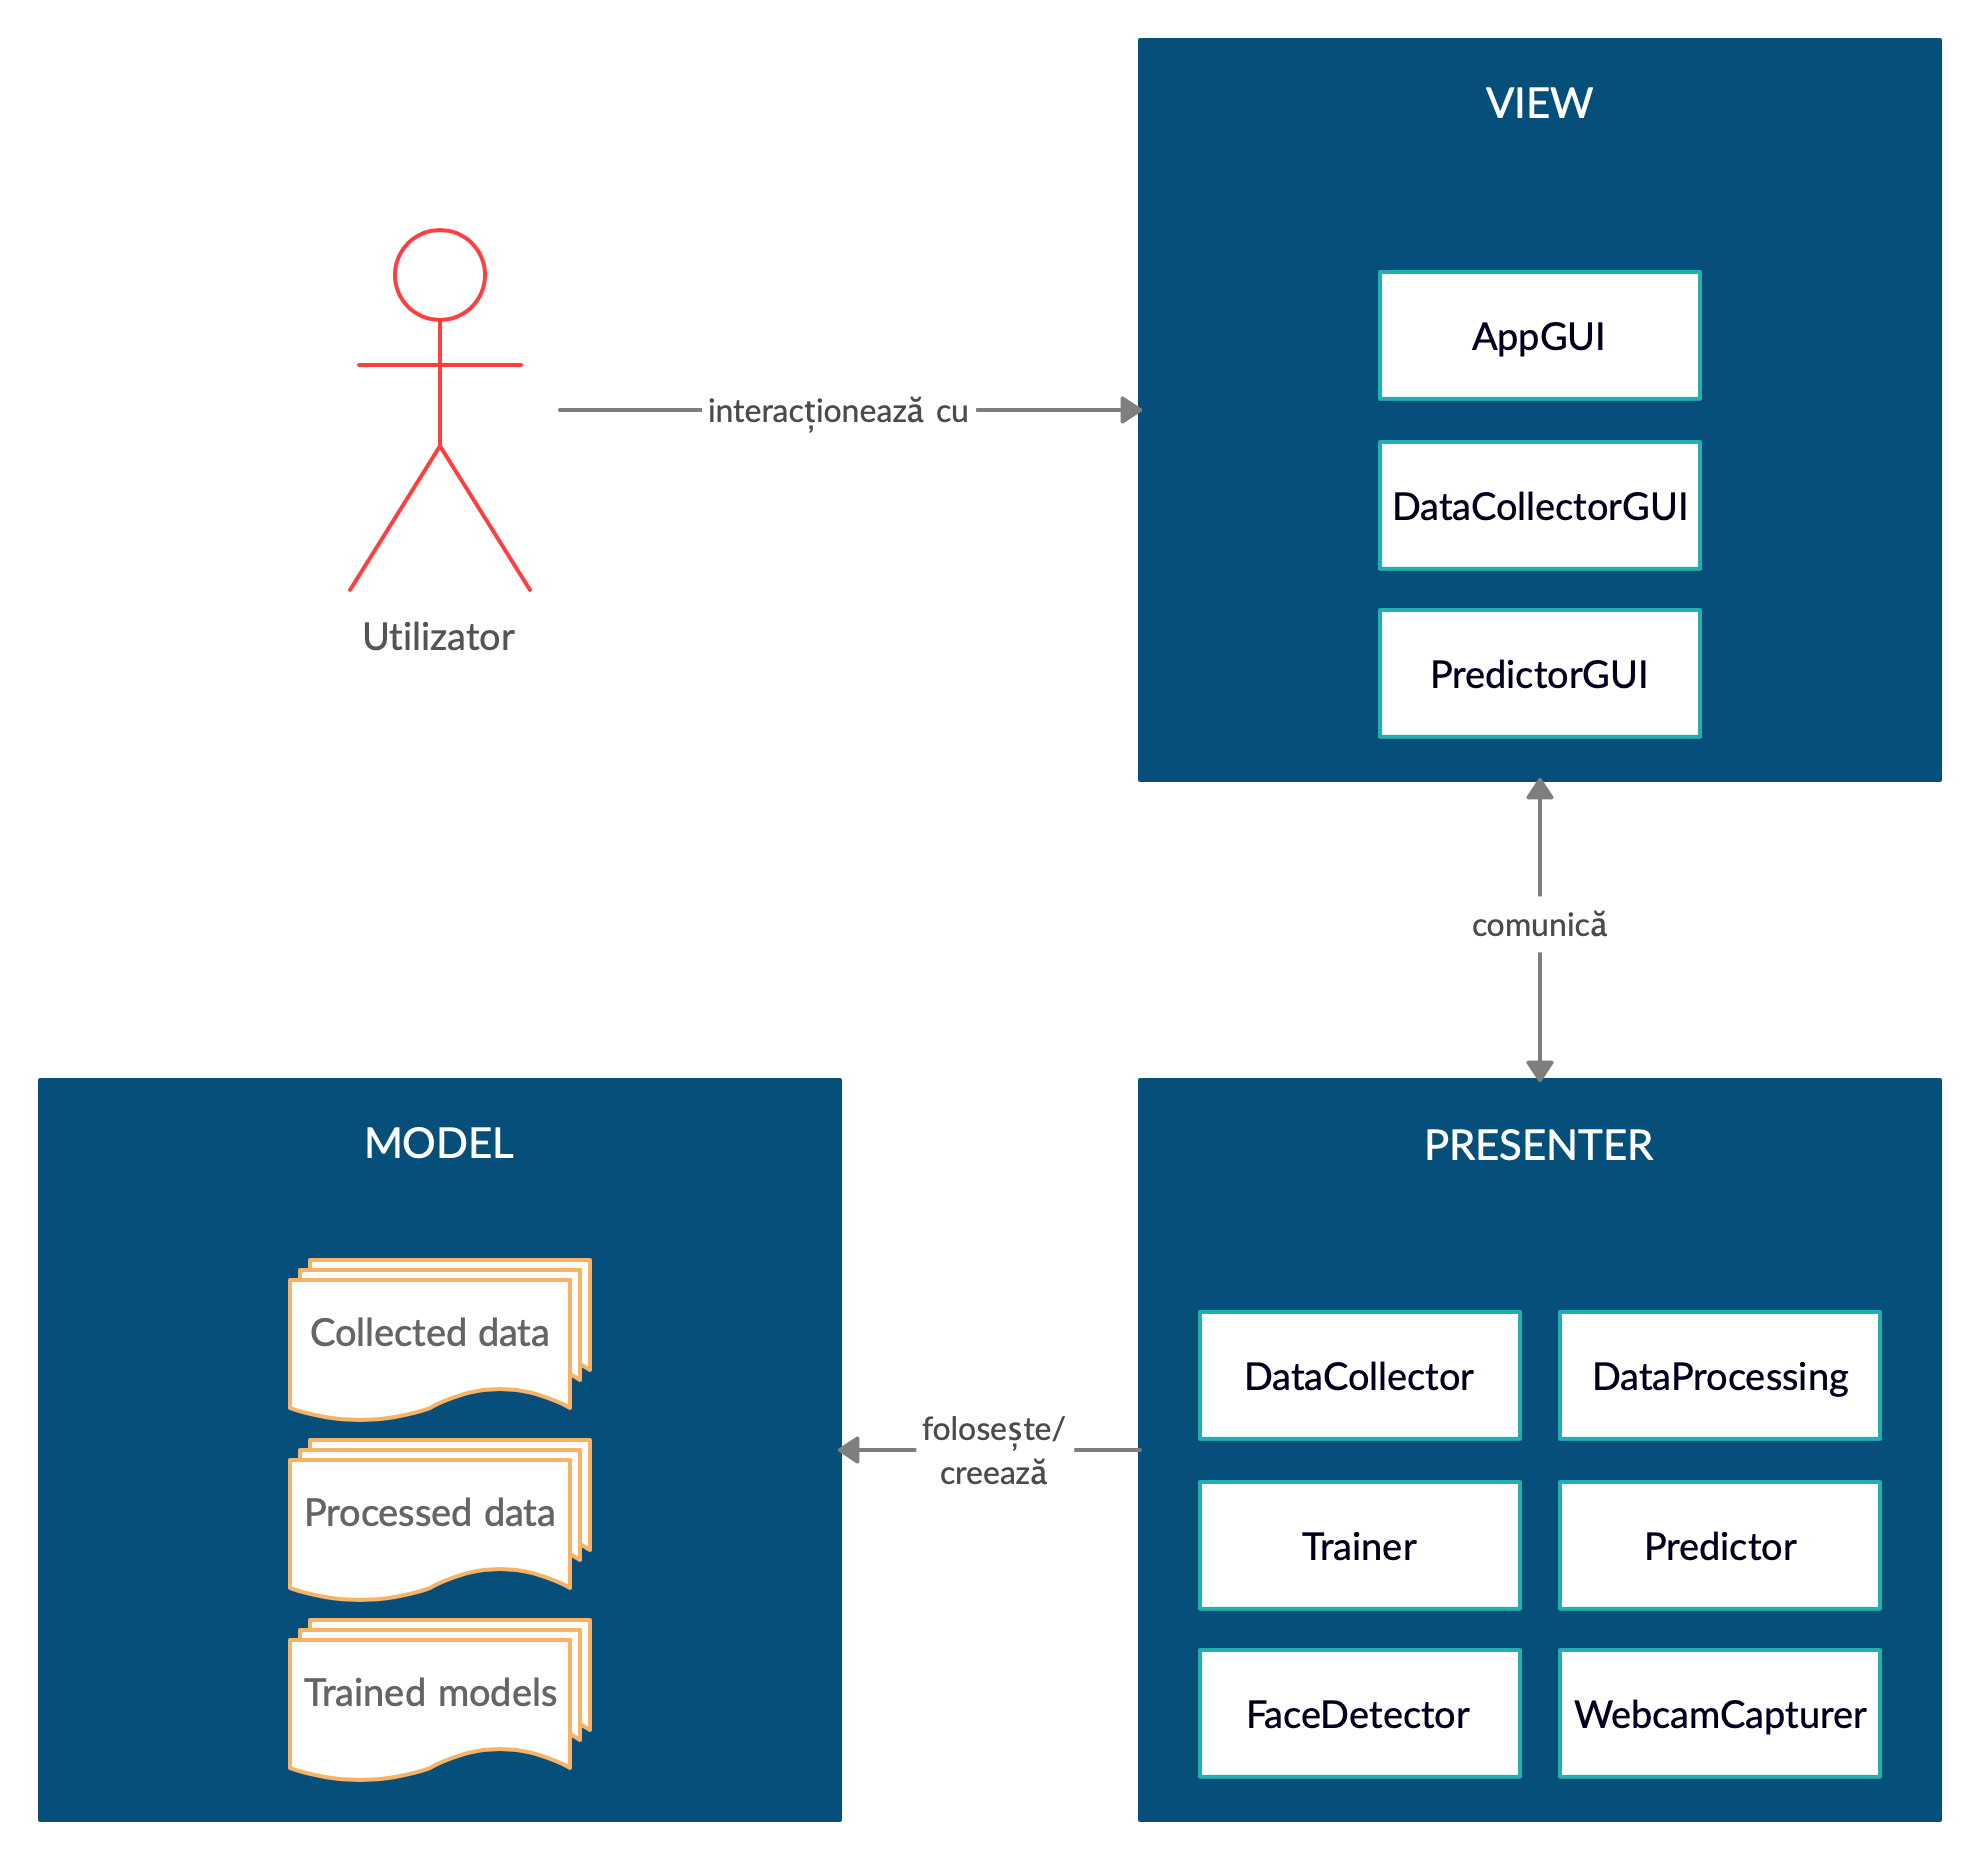
\includegraphics[width=\textwidth]{mvp.png}
    \caption{Arhitectura MVP a aplicației}
\end{figure}

\begin{figure}[ht]
    \centering
    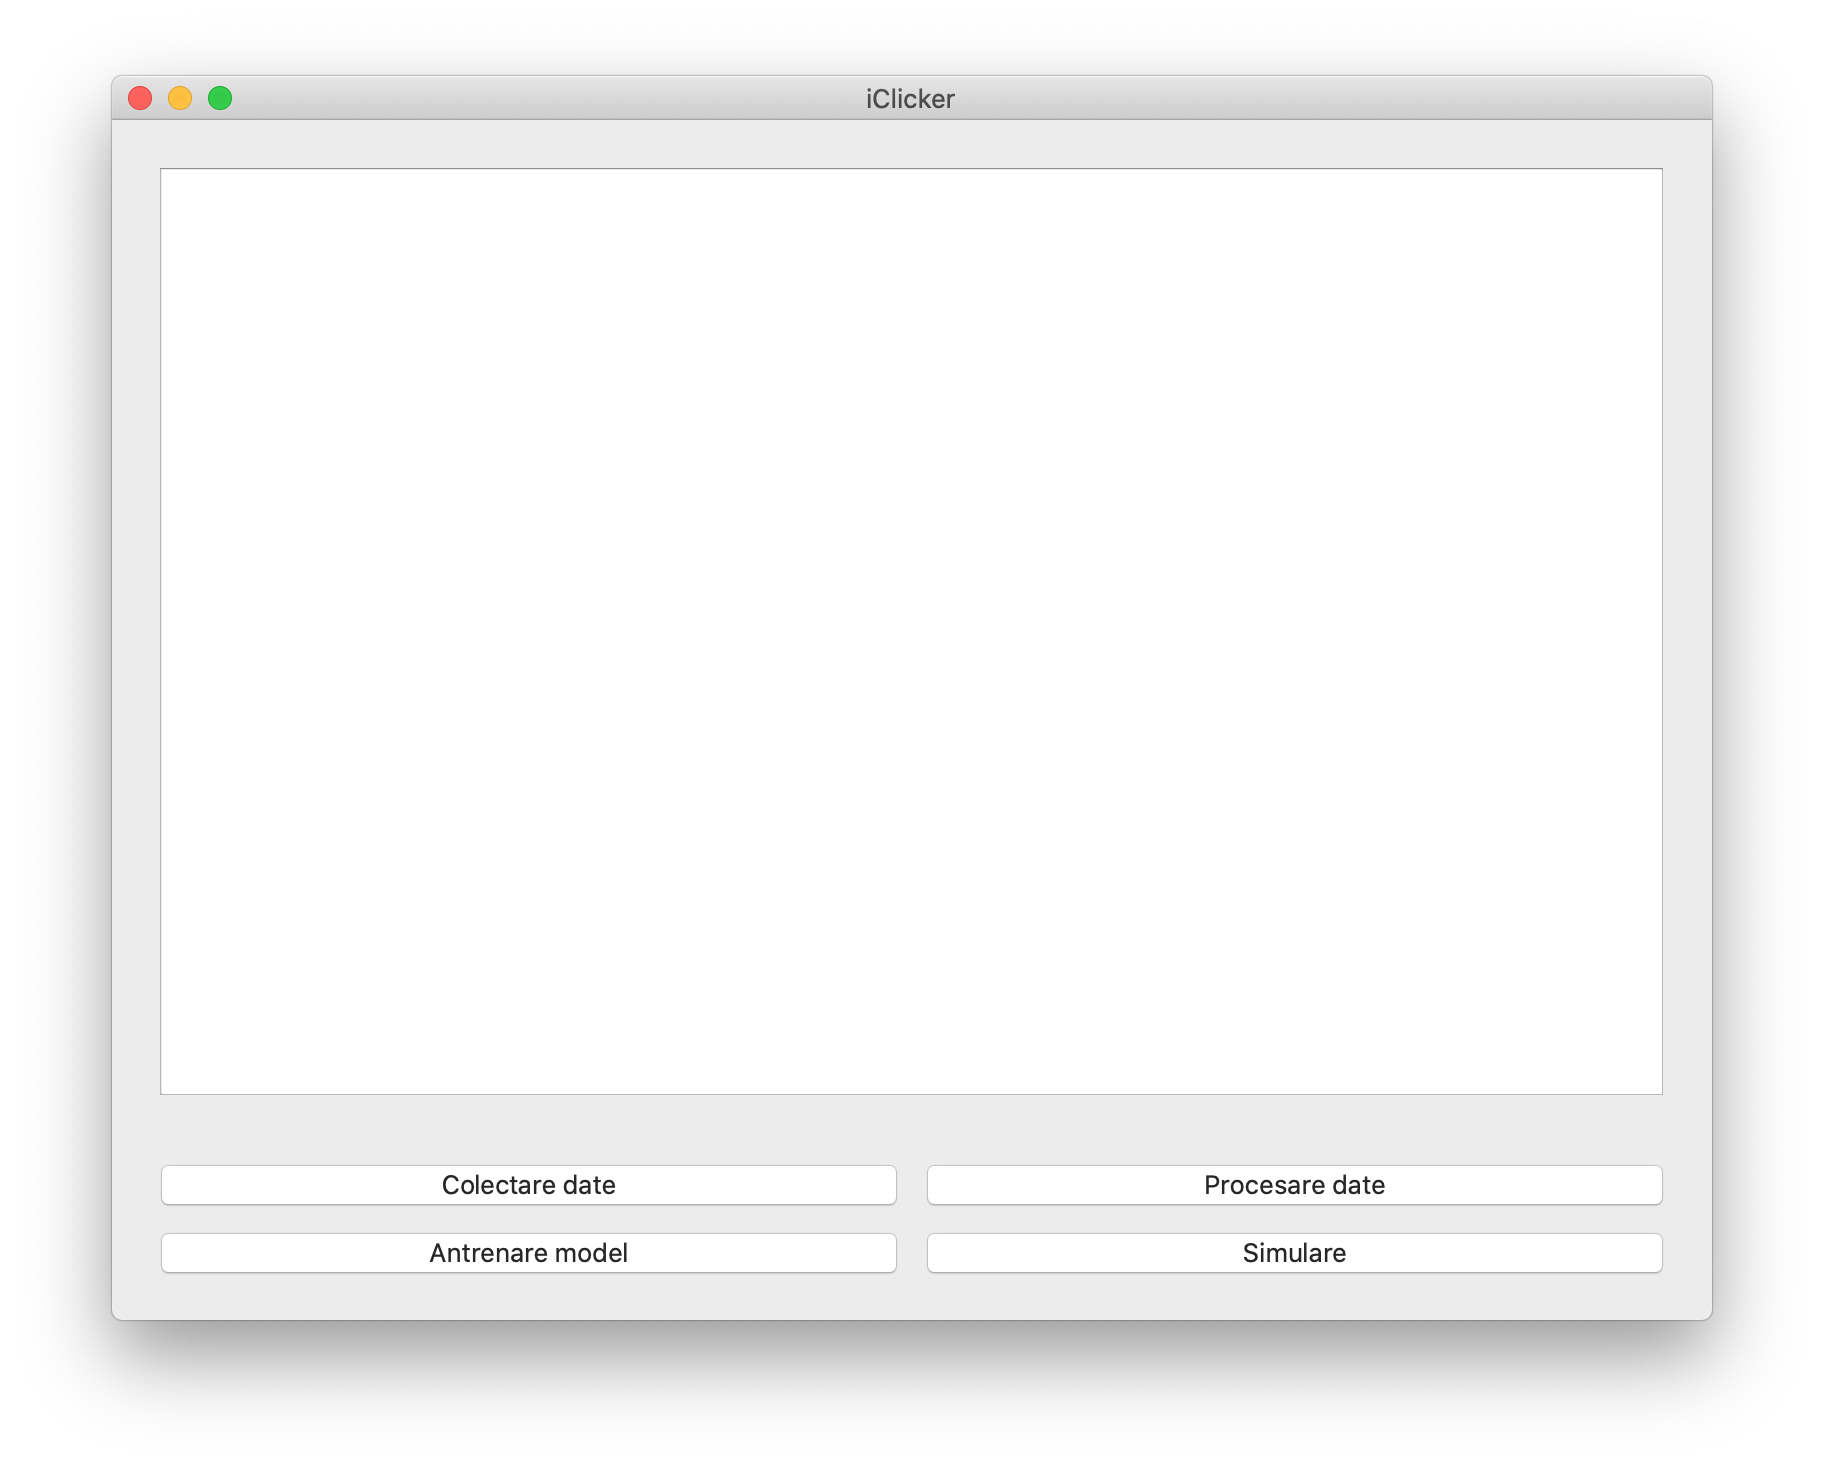
\includegraphics[width=\textwidth]{iClicker.png}
    \caption{Fereastra principală a aplicației}
\end{figure}

\begin{figure}[ht]
    \centering
    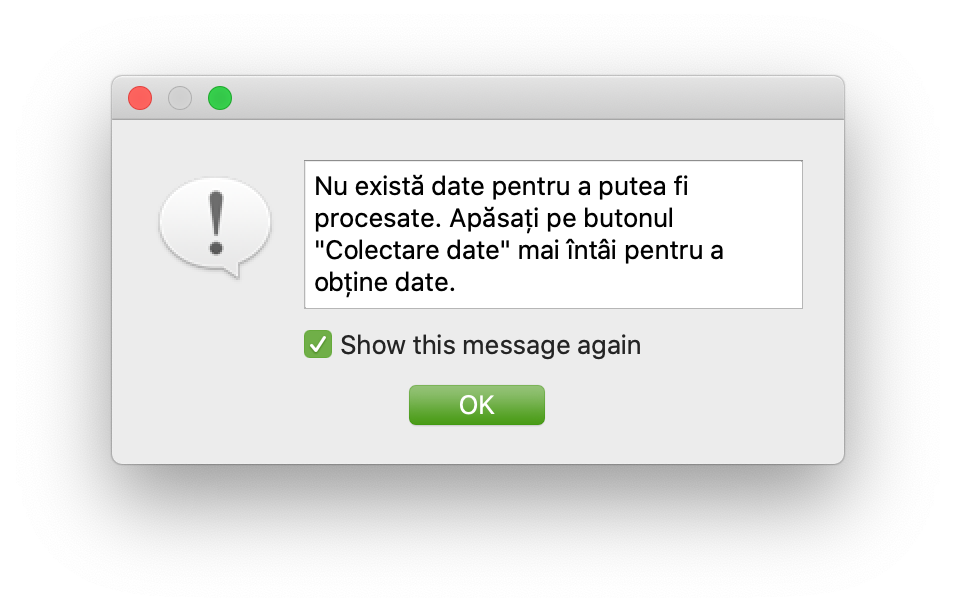
\includegraphics[width=0.32\textwidth]{err1.png}
    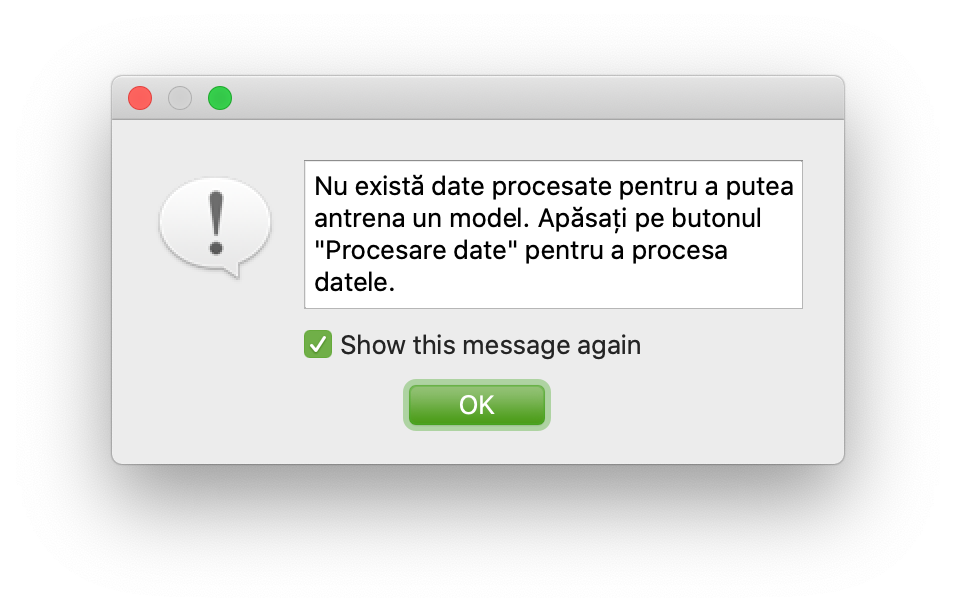
\includegraphics[width=0.32\textwidth]{err2.png}
    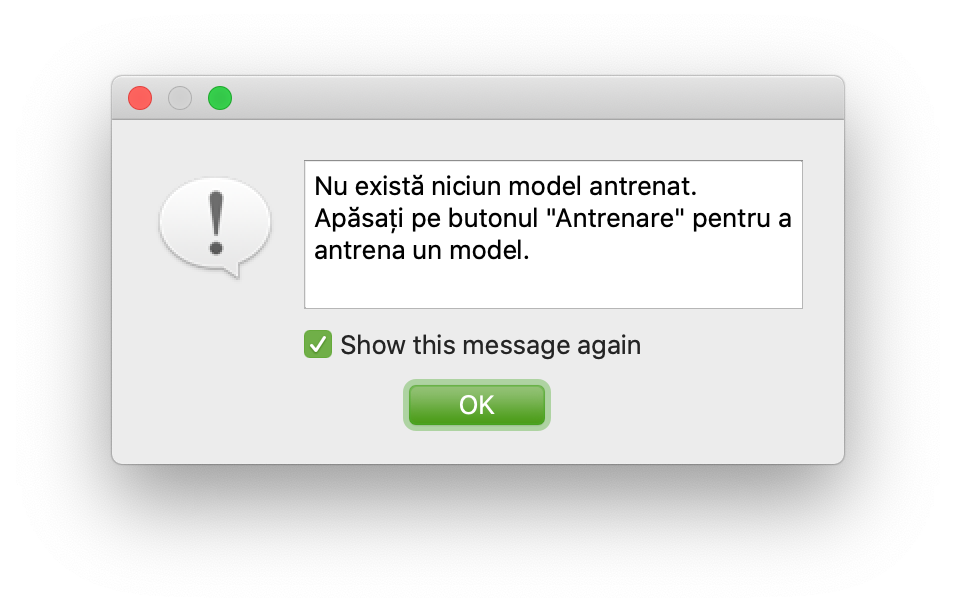
\includegraphics[width=0.32\textwidth]{err3.png}
    \caption{Mesaje de eroare}
\end{figure}

Pentru a realiza funcția de colectare a datelor, utilizatorul trebuie să apese pe butonul denumit sugestiv ``Colectare date''.
Există două moduri în care poate fi realizată această funcție: modul activ și modul pasiv.

Modul activ presupune ca utilizatorul să urmărească cursorul mouse-ului pe ecran în timp ce acesta se mișcă pe un traseu fix, prin mișcări glisante, de la stânga la dreapta, apoi de la dreapta la stânga, astfel încât să acopere toată suprafața ecranului.
De fiecare dată când cursorul își schimbă poziția, aplicația salvează o imagine preluată de la webcam împreună cu poziția cursorului în acel moment.
Pentru a evita obosirea ochilor și a asigura o colectare de date consistentă, utilizatorul poate lua o pauză (întreruperea mișcării cursorului și a colectării datelor) prin apăsarea tastei \emph{SPACEBAR}.
De asemenea, viteza cu care glisează cursorul poate fi schimbată prin apăsarea tastelor \emph{SĂGEATĂ SUS} și \emph{SĂGEATĂ JOS}.

Metoda pasivă este menită să nu deranjeze rutina utilizatorului, astfel încât de fiecare dată când utilizatorul apasă pe butonul stâng al mouse-ului, aplicația salvează, în același mod ca mai sus, o imagine capturată prin intermediul webcam-ului și poziția cursorului pe ecran.
Această variantă poate fi contraintuitivă, având în vedere că aplicația ar trebui folosită fără ajutorul mâinilor, dar m-a ajutat pe mine în obținerea datelor în timp ce realizam alte sarcini.
Este important de menționat că de multe ori nu ne uităm acolo unde apăsăm cu mouse-ul, așa că, deși este o metodă gândită să ruleze pe fundal, este bine ca utilizatorul să țină cont de prezența acesteia și să realizeze apăsări de buton acolo unde se uită, pentru a construi \emph{date consistente}.

Partea de procesare de date și de antrenare a modelelor se folosesc în același mod, prin apăsarea butoanelor denumite sugestiv.
Acestea vor informa utilizatorul despre progresul realizat prin intermediul ferestrei principale.

Toate aceste funcționalități rulează pe câte un \emph{fir de execuție} separat.
Dacă acest lucru nu s-ar petrece, atunci firul principal de execuție (care se ocupă și de afișarea componentelor grafice) ar fi ``blocat'' până la terminarea execuției acelor funcționalități și aplicația ar ``îngheța''.

Ultima componentă este și cea mai importantă, cea de simulare a funcționalităților mouse-ului.
Prin intermediul acesteia, aplicația începe să urmărească ochii utilizatorului și să-i analizeze gesturile faciale.
Utilizatorului i se va arăta pe ecran și o grilă (de dimensiune 3x3) pentru a vedea în timp real predicțiile rețelei convoluționale legate de zona ecranului pe care acesta o privește.

\begin{figure}[H]
    \centering
    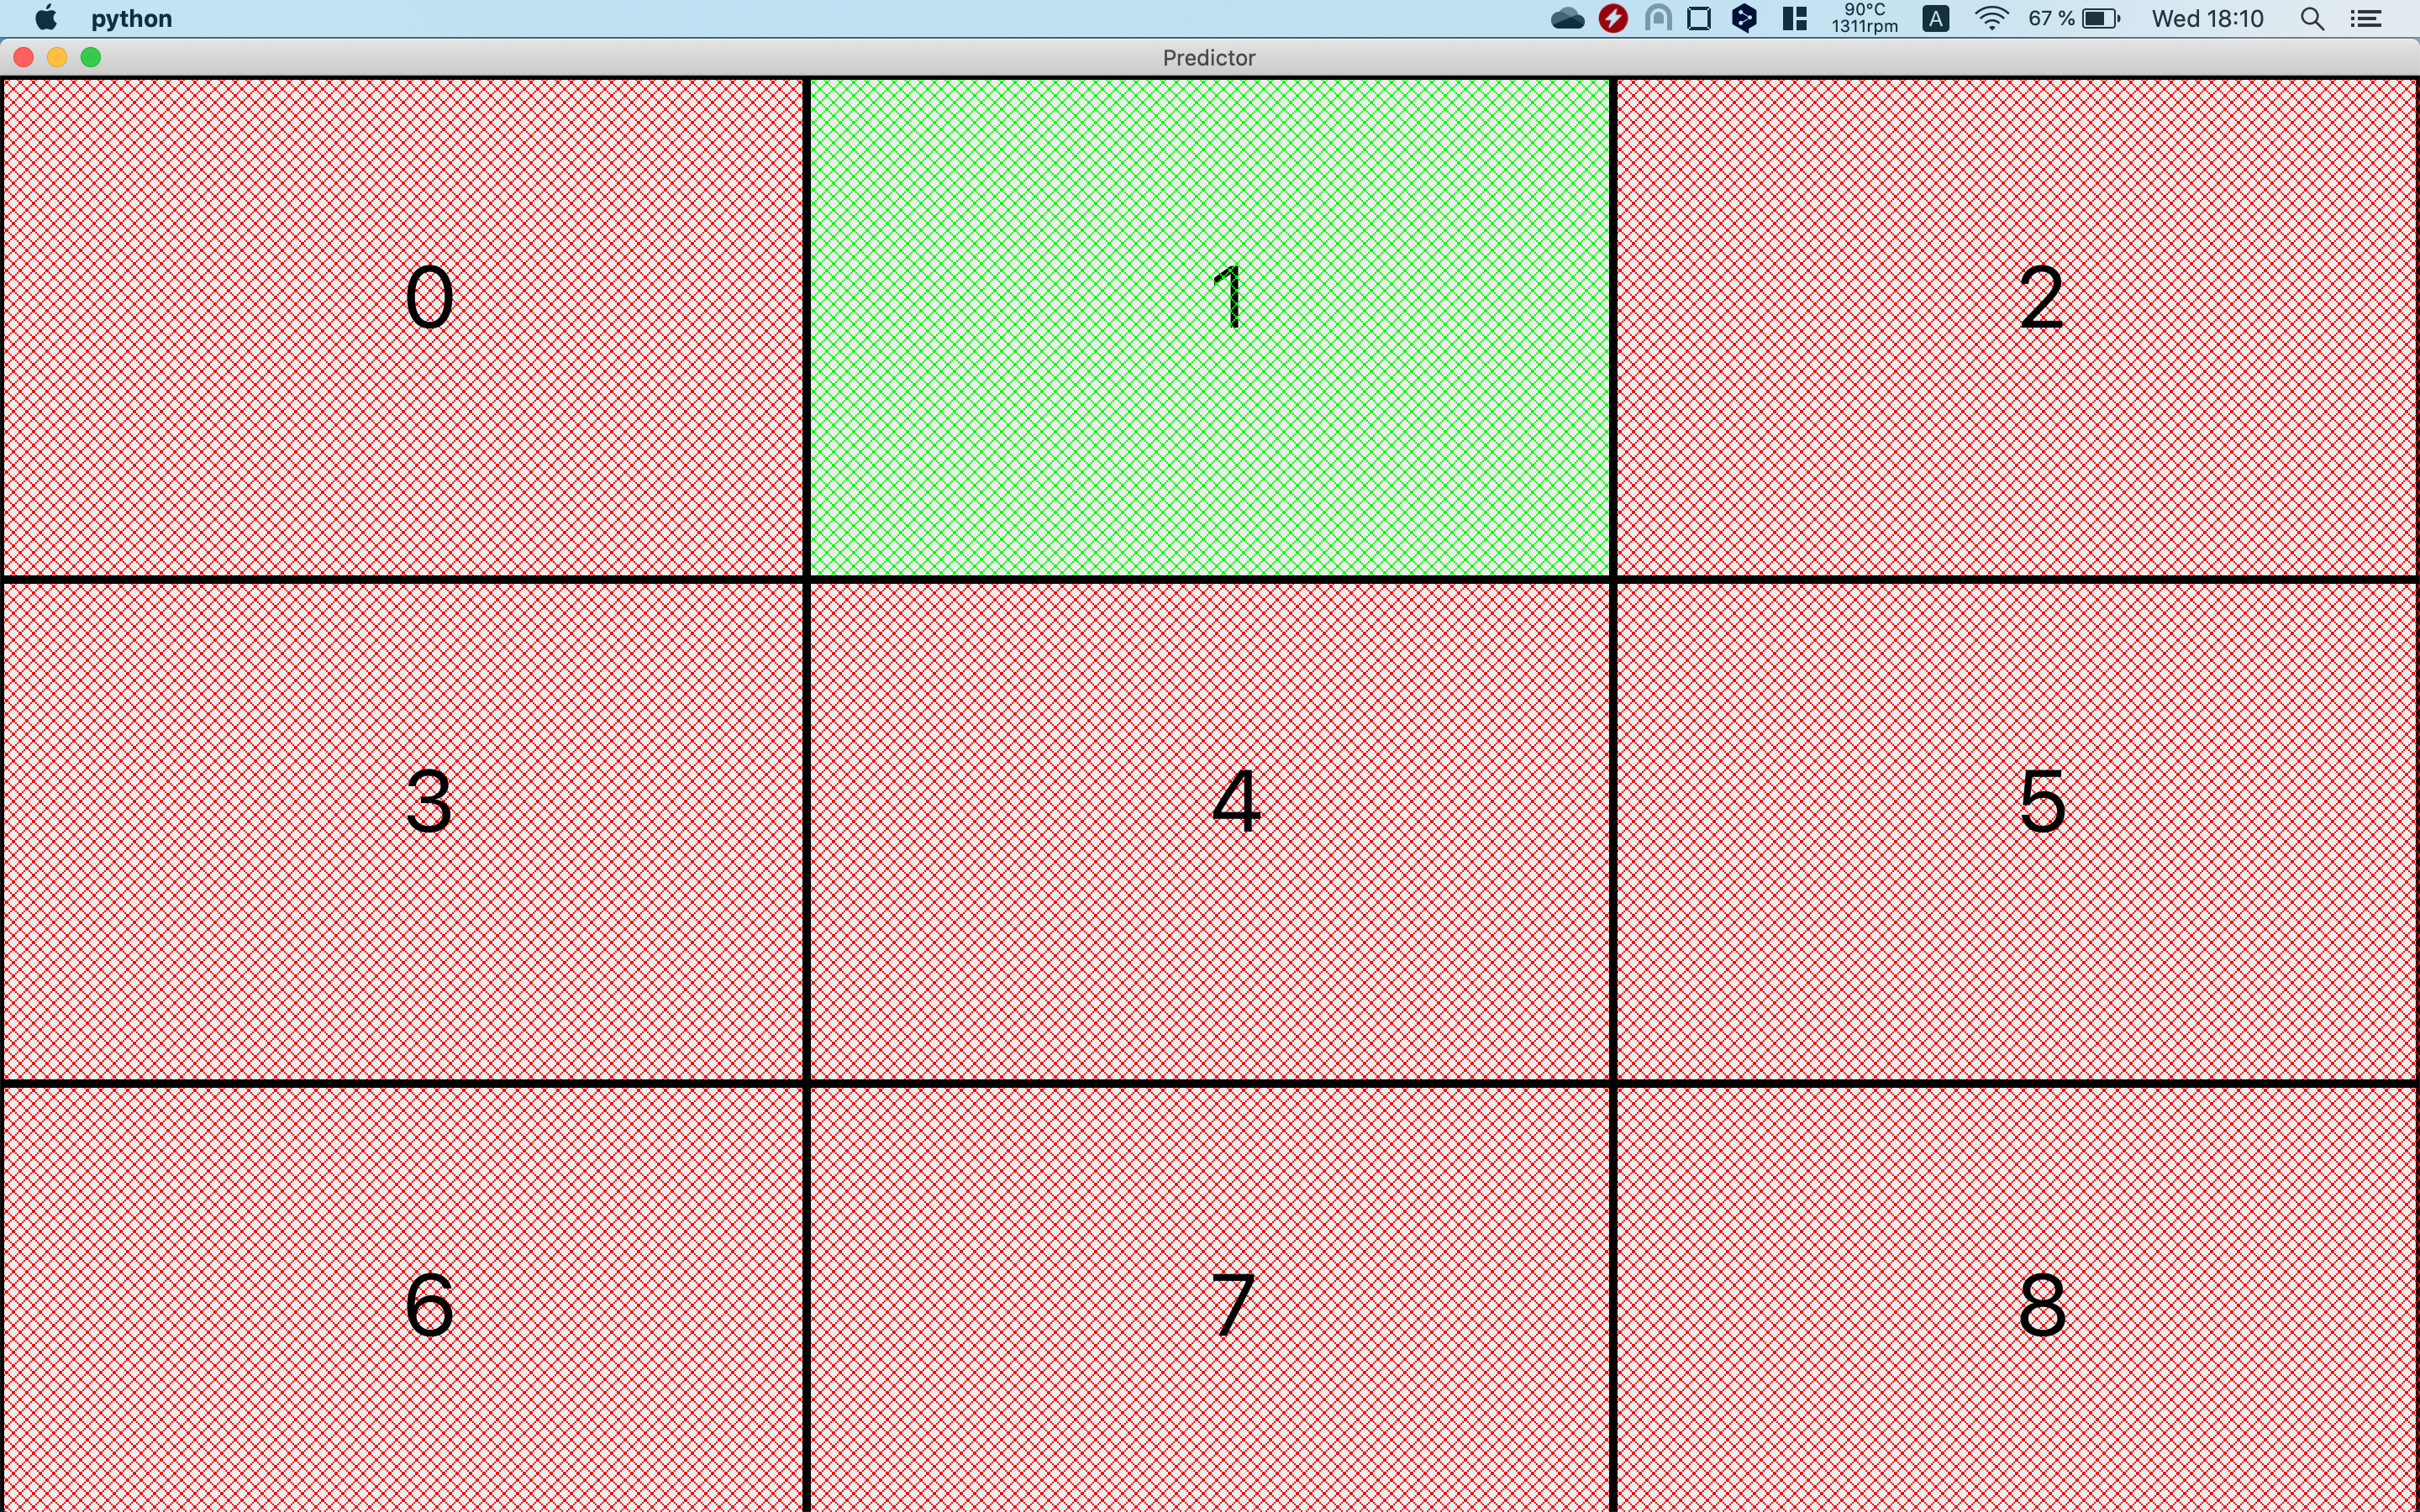
\includegraphics[width=0.49\textwidth]{pred1.png}
    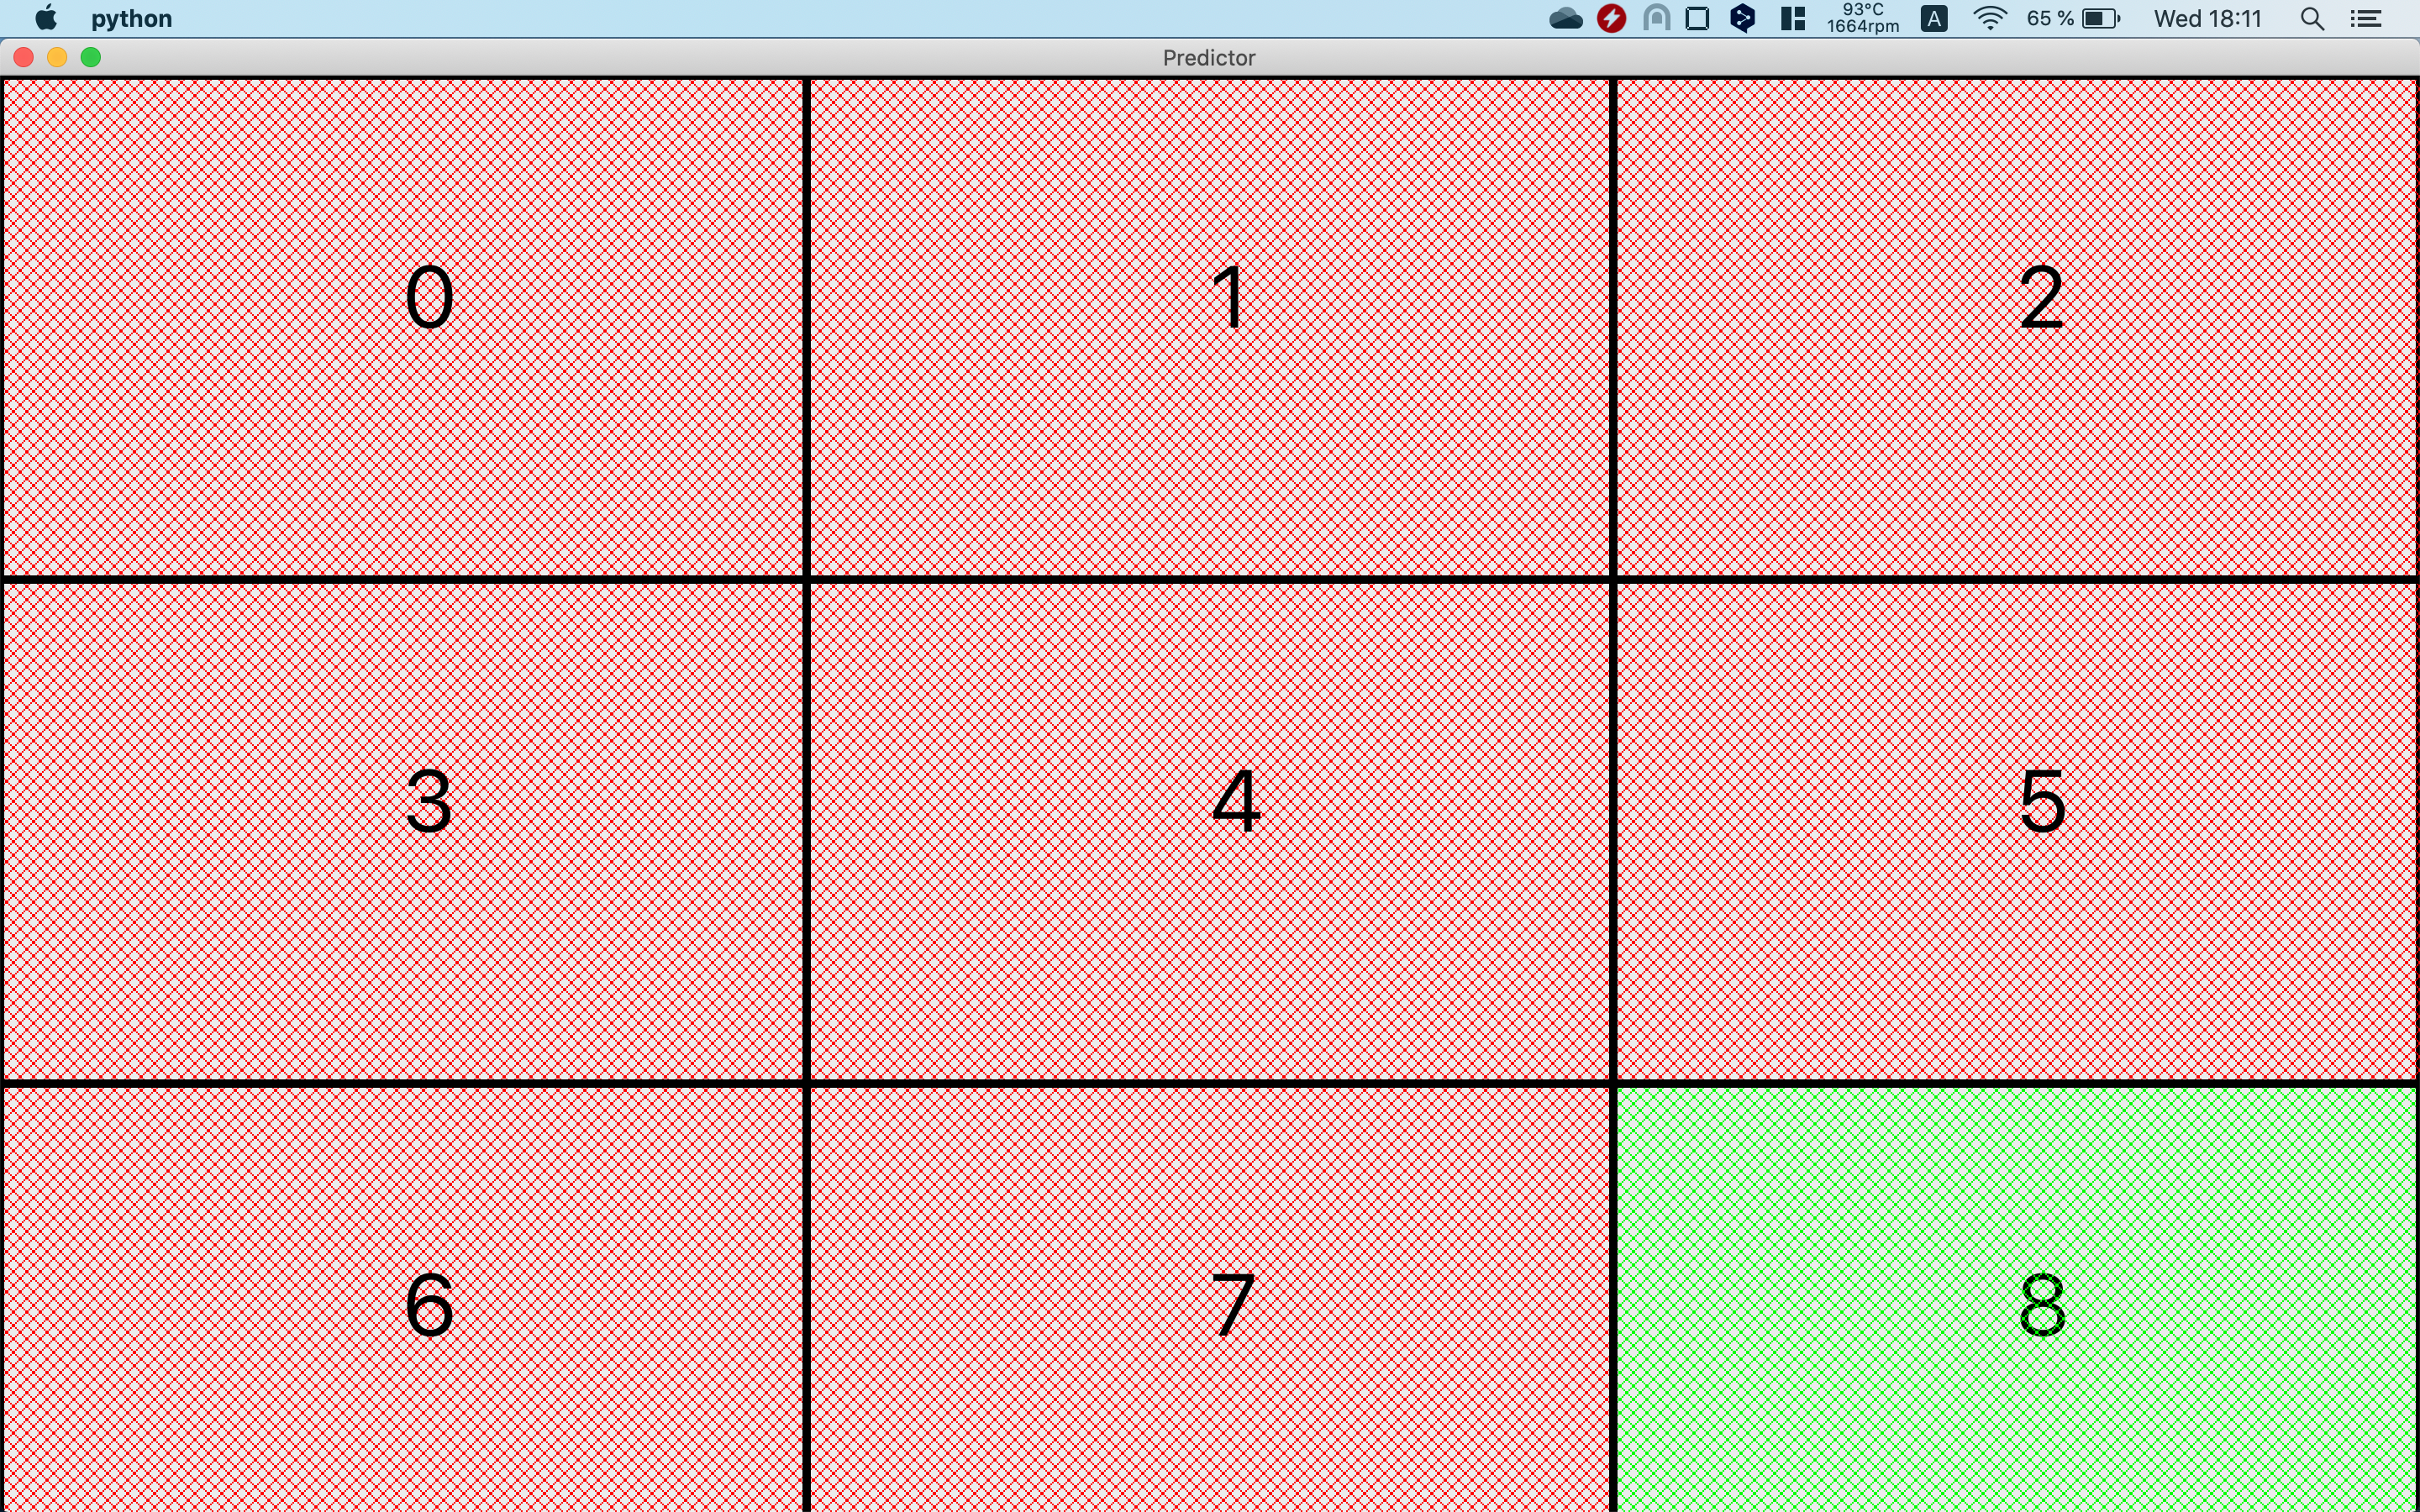
\includegraphics[width=0.49\textwidth]{pred2.png}
    \caption{Testarea predicțiilor ale zonei de privire ale utilizatorului}
\end{figure}

\begin{figure}[ht]
    \centering
    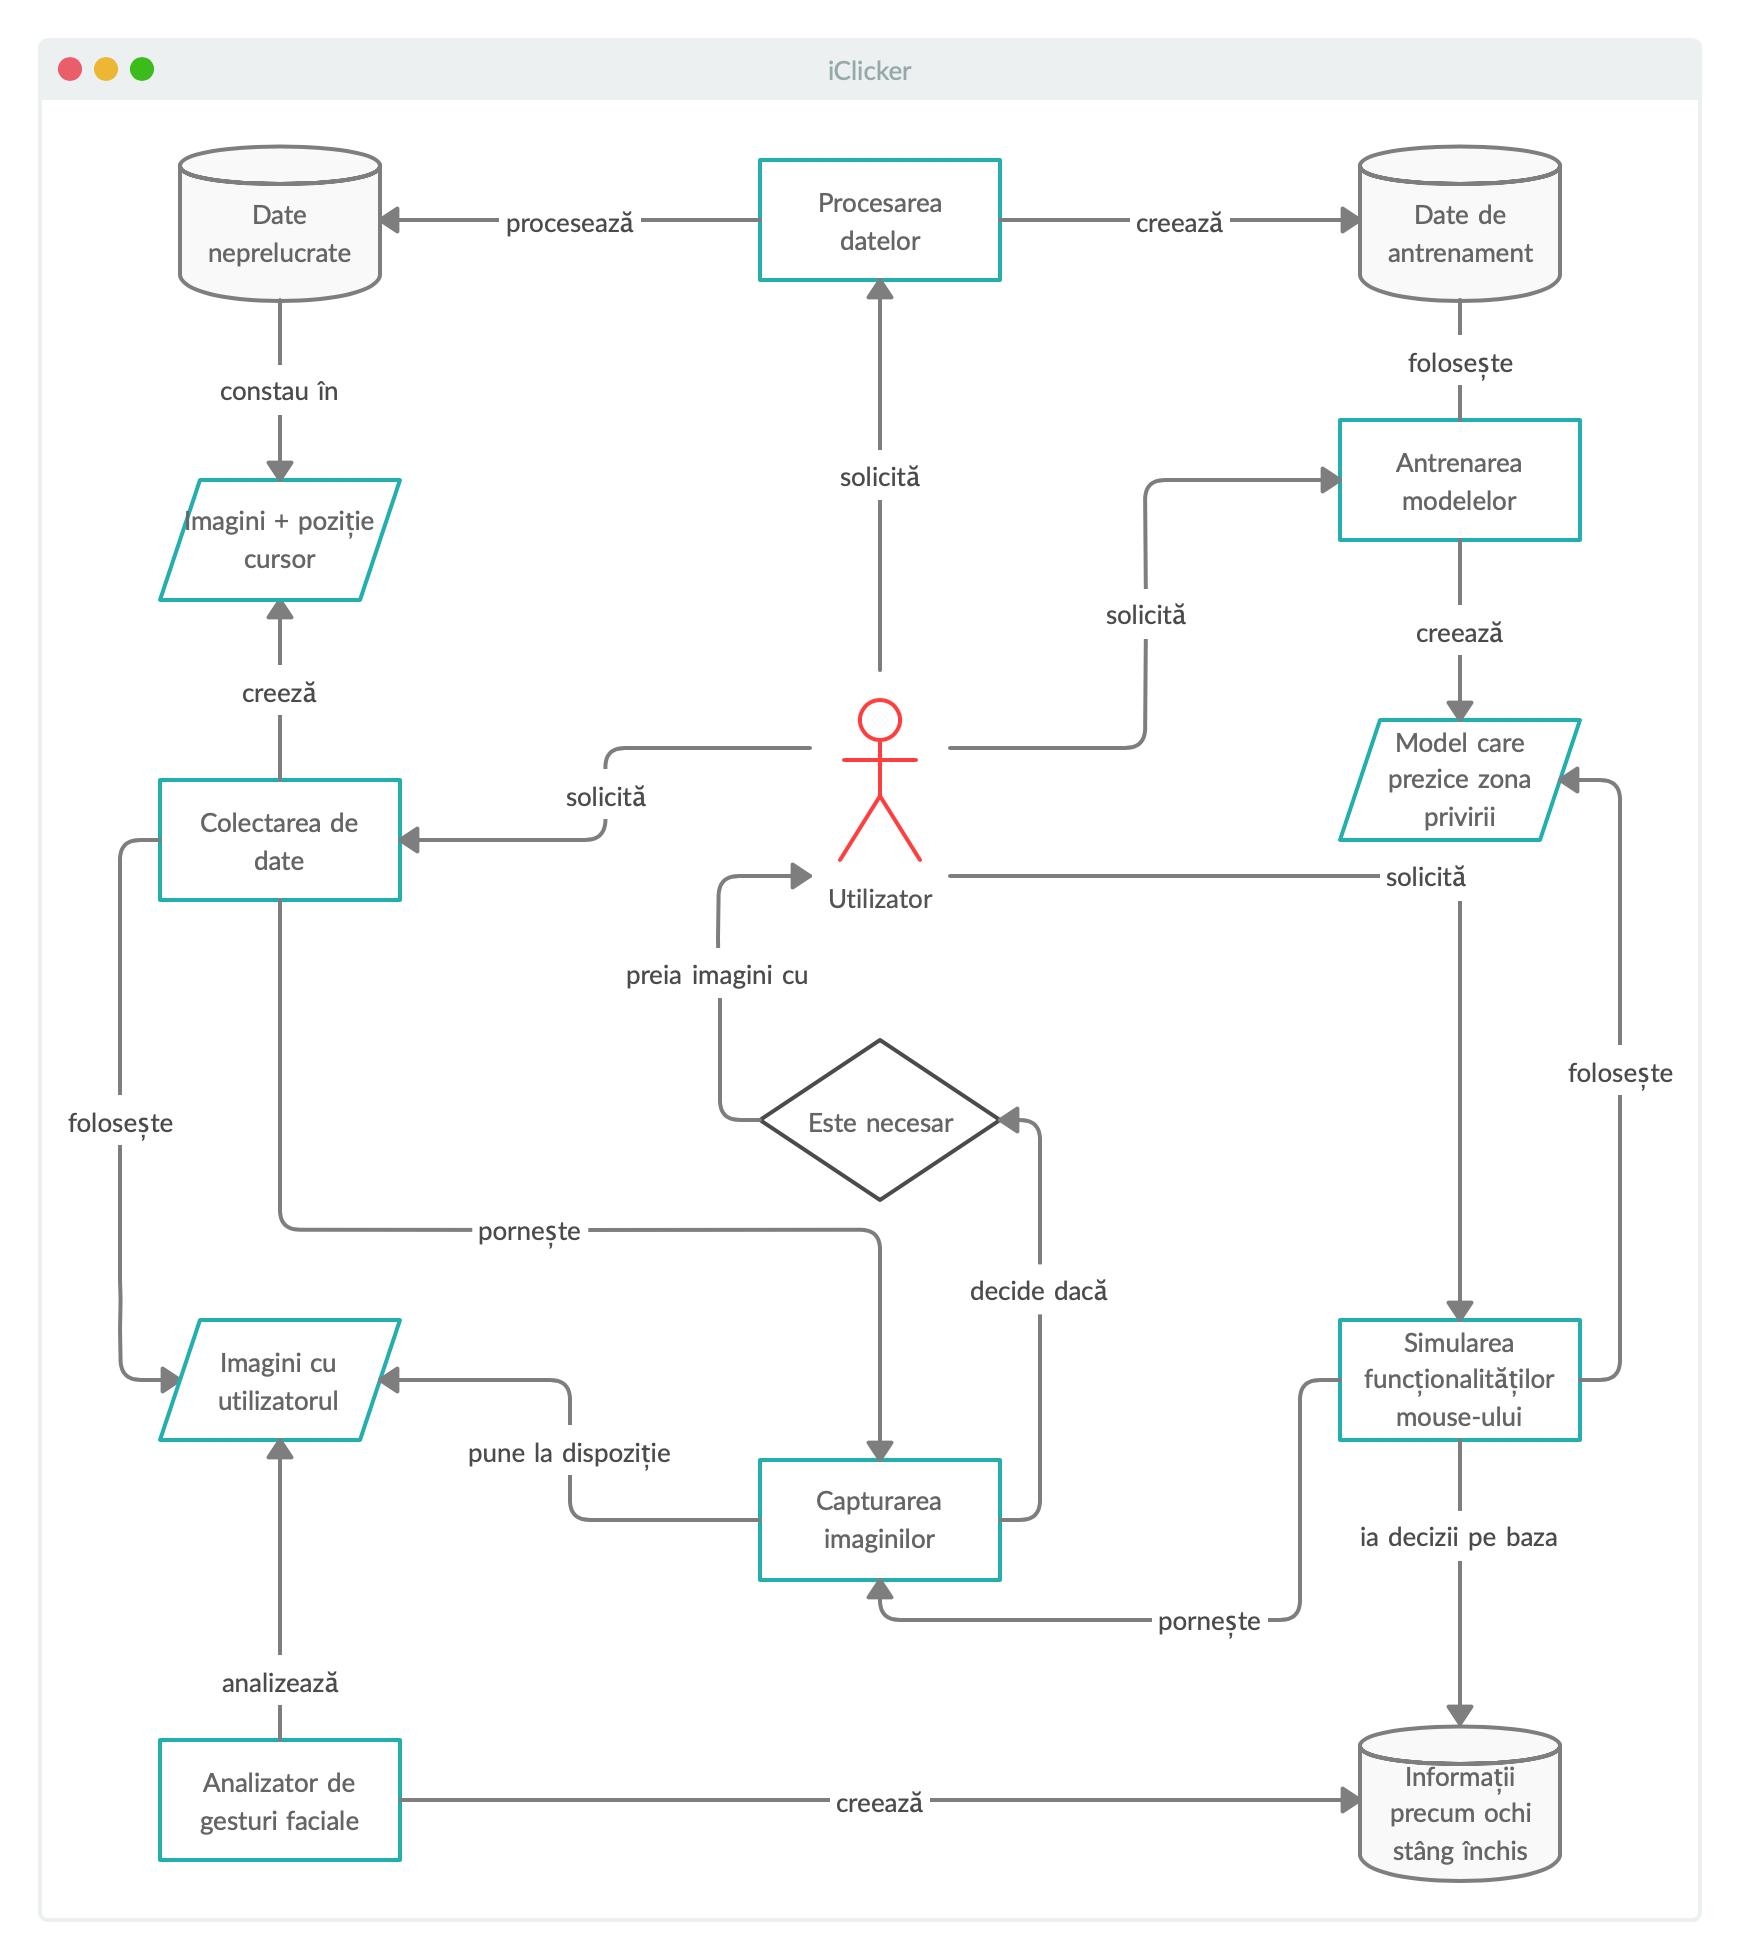
\includegraphics[width=\textwidth]{flowchart.png}
    \caption{Organigrama aplicației}
\end{figure}
